\section{Motivation and Requirement}
\label{sec:motivation-background}

The goal of our algorithm is to estimate the robot pose on the soccer field in the field coordinate system (FCS): position $x,y$ and orientation angle $\theta$. Observations are expressed in the robot coordinate system (RCS): motion observations such as speed and acceleration from odometry and IMU sensing, and visible landmarks such as goals, corners, line intersections, and the center circle. With this information, the current belief represented in red in Fig.~\ref{fig:localization-requirement} must find the actual robot pose generating the observations in green.

\begin{figure}[!htbp]
    \centering
    \begin{minipage}[c]{0.45\linewidth}
        \centering
        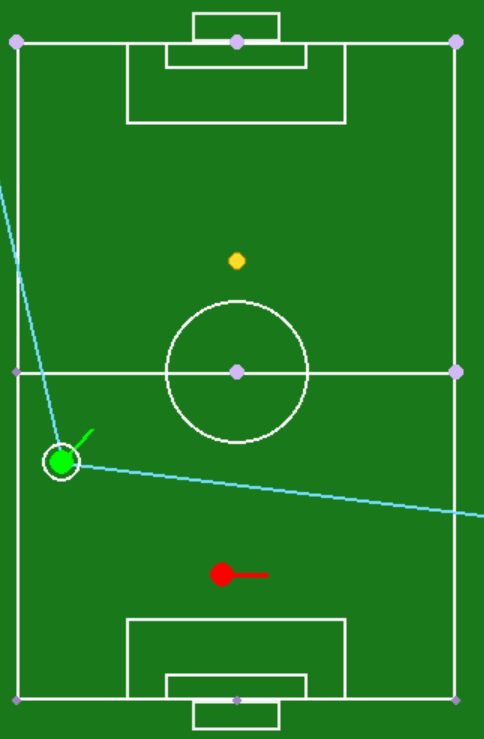
\includegraphics[width=0.58\linewidth]{figures/Soccer_field.png}
    \end{minipage}
    \hfill
    \begin{minipage}[c]{0.45\linewidth}
        \centering
        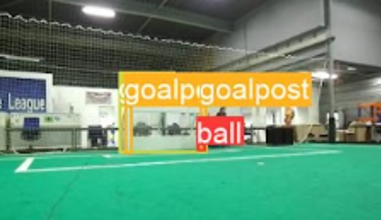
\includegraphics[width=0.62\linewidth]{figures/landmark1.png}\\[0.3em]
        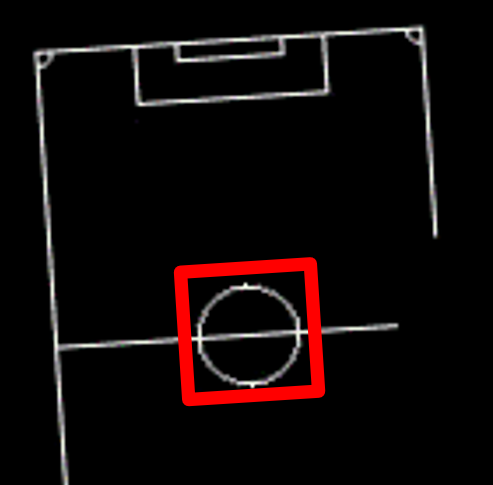
\includegraphics[width=0.25\linewidth]{figures/landmark2.png}
    \end{minipage}
    \caption{Robot-soccer localization requirement. The belief in red must converge to the actual pose generating the observations in green, using motion observations and visible landmarks as purple dots inside the limited field of view. Typical landmark examples include goal posts and the middle circle; the landmark center $(x,y)$ in RCS is used as input to the algorithm.}
    \label{fig:localization-requirement}
\end{figure}
This must be done for fast-moving robots, reaching speeds up to 5 m/s and accelerations up to 12 m/s$^2$. It must provide robust, centimeter-scale tracking despite noisy, partial, intermittent, and ambiguous landmark observations, including temporary obstruction and a restricted 110-degree field of view. The restricted field of view reflects RoboCup's evolution toward humanoid robot soccer, where omnivision cameras are not available, in line with RoboCup's long-term objective of developing fully autonomous humanoid robot soccer players capable of defeating the human World Cup champion by the middle of the 21st century~\cite{robocup_objective_2026}.
The method leverages the fact that robot soccer is played on a known field: landmarks are specified upfront and do not need to be learned, and the transformations between the robot coordinate system (RCS) and field coordinate system (FCS) are known.

\FloatBarrier
